\chapter{Formáty uložení řídkých matic}

% http://www.cs.colostate.edu/~mroberts/toolbox/c++/sparseMatrix/sparse_matrix_compression.html

Formáty uložení řídkých matic obecně ukládají jednotlivé prvky zvlášť, a tedy nemusí ukládat ty nulové. To ale přináší řadu nevýhod. Za prvé se musí ukládat informace o souřadnicích a za druhé ztrácíme možnost přístupu k prvku na libovolných souřadnicích v čase $\Theta(1)$, protože prvky nemáme přímo indexované podle jejich umístění v řádku a sloupci.

Protože řídké matice můžeme rozdělit do mnoha kategorií a provádět nad nimi mnoho operací, existuje mnoho formátů, jak řídkou matici efektivně uložit a pracovat s ní. Formáty uložení řídkých matic můžeme také rozdělit podle toho, zdali je možné do nich přidávat nebo z nich odebírat prvky.

Při násobení matic $C = A \cdot B$ se matice $A$ ani $B$ nemění. V této práci budeme předpokládat, že matice $C$ bude hustá a formáty umožňující přidávání nebo odebírání prvků nebudou součástí práce. Stejně tak při násobení matice $A$ vektorem $B$ je výsledek $C$ vektor.

Dalším kritériem pro rozdělení formátů je uspořádanost nenulových prvků v řídké matici. Pro uspořádané matice bude efektivnější takový formát, který využije určitý vzor, v jakém jsou prvky matice uloženy. V řídkých maticích takovým vzorem může být například diagonála nebo blok prvků. Efektivně lze za vzor považovat i prvky v řádku nebo ve sloupci.

Uspořádáním může být také symetrie matice, kdy nám stačí uložit pouze polovinu matice. Často bývají řídké matice symetrické podle hlavní diagonály.

\section{COO - Coordinate list}

Formát COO, česky seznam souřadnic, je základní formát řídkých matic. Ke~každému nenulovému prvku ukládá jeho souřadnice \texttt{y} a \texttt{x}. Implementovat tento formát můžeme například jako tři pole. Pole \texttt{v} s hodnotami prvků, pole \texttt{r} s \texttt{y} souřadnicemi a pole \texttt{c} s \texttt{x} souřadnicemi.

Pro ukázku v tomto formátu uložíme matici o velikosti $n=8$ s $nnz=5$ nenulovými prvky.

\begin{align}
\begin{pmatrix}
	0 & 0 & 0 & 0 & 0 & 0 & 0 & 0 \\
	\boldsymbol{1} & \boldsymbol{2} & 0 & 0 & 0 & 0 & 0 & 0 \\
	0 & 0 & 0 & 0 & 0 & 0 & 0 & 0 \\
	0 & 0 & 0 & 0 & 0 & 0 & 0 & 0 \\
	0 & \boldsymbol{3} & 0 & 0 & 0 & 0 & 0 & 0 \\
	0 & 0 & 0 & 0 & 0 & 0 & 0 & 0 \\
	0 & 0 & 0 & 0 & 0 & \boldsymbol{4} & \boldsymbol{5} & 0 \\
	0 & 0 & 0 & 0 & 0 & 0 & 0 & 0 \\	
\end{pmatrix} \notag
\end{align}

\begin{table}[htb]
    \begin{tabular}{r|lllll}
    values[5]   & 1 & 2 & 3 & 4 & 5 \\
    y-coords[5] & 1 & 1 & 4 & 7 & 7 \\
    x-coords[5] & 0 & 1 & 1 & 5 & 6 \\
    \end{tabular}
    \caption{Matice uložená ve formátu COO}
\end{table}

Jak můžeme vidět, délka polí je závislá pouze na $nnz$. Pro velké matice s malým počtem neuspořádaných nenulových prvků je tento formát velmi efektivní. Pokud by bylo prvků velké množství, informace o uložení \texttt{y} nebo \texttt{x} souřadnic by byla často redundantní.

Paměťová náročnost formátu COO je $O(3 \cdot nnz)$.

Formát COO je velmi jednoduchý a přímočarý. Při procházení jeho prvků nám stačí jedna iterace přes tři stejně dlouhá pole. Tím je tedy například algoritmus násobení řídké matice ve formátu COO s vektorem velmi jednoduchý:

\begin{algorithm}[htb]
	\caption{Násobení matice COO s vektorem}\label{coo-mvm}
	\begin{algorithmic}[1]
		\Procedure{COO-MVM}{COO,V,C}
		\For{\texttt{i$\gets$0\TO COO.nnz}}
			\State \texttt{V.v[COO.r[i]] += COO.v[i] * V.v[COO.c[i]];	}
		\EndFor
		\EndProcedure
	\end{algorithmic}
\end{algorithm}

\label{alg:coo-mmm}
Při násobení dvou matic narazíme na problém. Při této operaci se každý prvek násobí dvakrát. Potřebujeme způsob, jak se v matici vrátit zpátky na určité místo. Takový naivní algoritmus pro násobení dvou COO matic by byl složitý. Museli bychom si pamatovat začátky řádků a neustále kontrolovat, jestli jsme nepřesáhli další řádek. Lepším řešením je dopředu si předpočítat, kde který řádek začíná a končí. Předpočítáme si tedy pole, nazvané $row\_pointers$, o délce $M.height + 1$, obsahující indexy začátků a konců řádek.

Při procházení matice se tak v poli s prvky mezi indexy $row\_pointers[i]$ a $row\_pointers[i+1]$ nachází prvky na řádku $i$. Proto je pole právě o jedna delší než výška matice, abychom mohli určit konec posledního řádku.

\begin{algorithm}[htb]
	\caption{Násobení dvou COO matic}\label{coo-mmm}
	\begin{algorithmic}[1]
		\Procedure{COO-MMM}{A,B,C}
		\State \texttt{arp $\gets$ ComputeRowBeginnings(A, A.nnz + 1);}
		\State \texttt{brp $\gets$ ComputeRowBeginnings(B, B.nnz + 1);}
		\For{\texttt{i $\gets$ 0\TO A.height}}\Comment{násobení}
			\For{\texttt{ac$\gets$arp[i]\TO arp[i + 1]}}
				\For{\texttt{bc$\gets$brp[A.c[ac]]\TO brp[A.c[ac] + 1]}}
					\State \texttt{C.v[r][A.c[bc]] += A.v[ac] * B.v[bc];}
				\EndFor
			\EndFor
		\EndFor
		\EndProcedure
	\end{algorithmic}
\end{algorithm}

V části s násobením již pole s \texttt{y} souřadnicemi nepotřebujeme. Lepší formát uložení řídkých matic pro násobení by byl takový, který namísto pole s \texttt{y} souřadnicemi obsahuje předpočítané začátky a konce řádků. Takovým formátem je CSR.

%%%%%%%%%%%%%%%%%%%%%%%%%%%%%%%%%%%%%%%%%%%%%%%%%%%%%%%%%%%%%%%%%%%%%%%%%%%%%%
%%%%%%%%%%%%%%%%%%%%%%%%%%%%%%%%%%%%%%%%%%%%%%%%%%%%%%%%%%%%%%%%%%%%%%%%%%%%%%
%%%%%%%%%%%%%%%%%%%%%%%%%%%%%%%%%%%%%%%%%%%%%%%%%%%%%%%%%%%%%%%%%%%%%%%%%%%%%%
%%%%%%%%%%%%%%%%%%%%%%%%%%%%%%%%%%%%%%%%%%%%%%%%%%%%%%%%%%%%%%%%%%%%%%%%%%%%%%
%%%%%%%%%%%%%%%%%%%%%%%%%%%%%%%%%%%%%%%%%%%%%%%%%%%%%%%%%%%%%%%%%%%%%%%%%%%%%%
%%%%%%%%%%%%%%%%%%%%%%%%%%%%%%%%%%%%%%%%%%%%%%%%%%%%%%%%%%%%%%%%%%%%%%%%%%%%%%

\subsection{Formát MatrixMarket}
\label{mtxsubsect}

MatrixMarket \cite{Boisvert:1997:MMW:265834.265854} je internetová sada matic s vlastním formátem pro uložení řídkých matic \texttt{.mtx}. Tato sada obsahuje skoro pět set matic z různých oblastí. Obsahuje i generátory řídkých matic, jejichž výstupy jsou matice různých vlastností.

Formát MatrixMarket se velmi podobá formátu COO. Navíc umožňuje nastavit matici jako symetrickou a uložit pouze její polovinu.

\section{CSR - Compressed sparse row}

Problém efektivnosti formátu COO pro větší množství prvků řeší formát CSR, česky komprimované řídké řádky. Formát CSR obsahuje pole $row\_pointers$, které ukládá informace o tom, kolik se v daném řádku nachází prvků, tedy to, co jsme si předpočítali v algoritmu \ref{coo-mmm}. K poli s hodnotami je další pole $col\_indices$, přiřazující ke každému prvku informaci o sloupci.

\begin{figure}[htb]\centering
	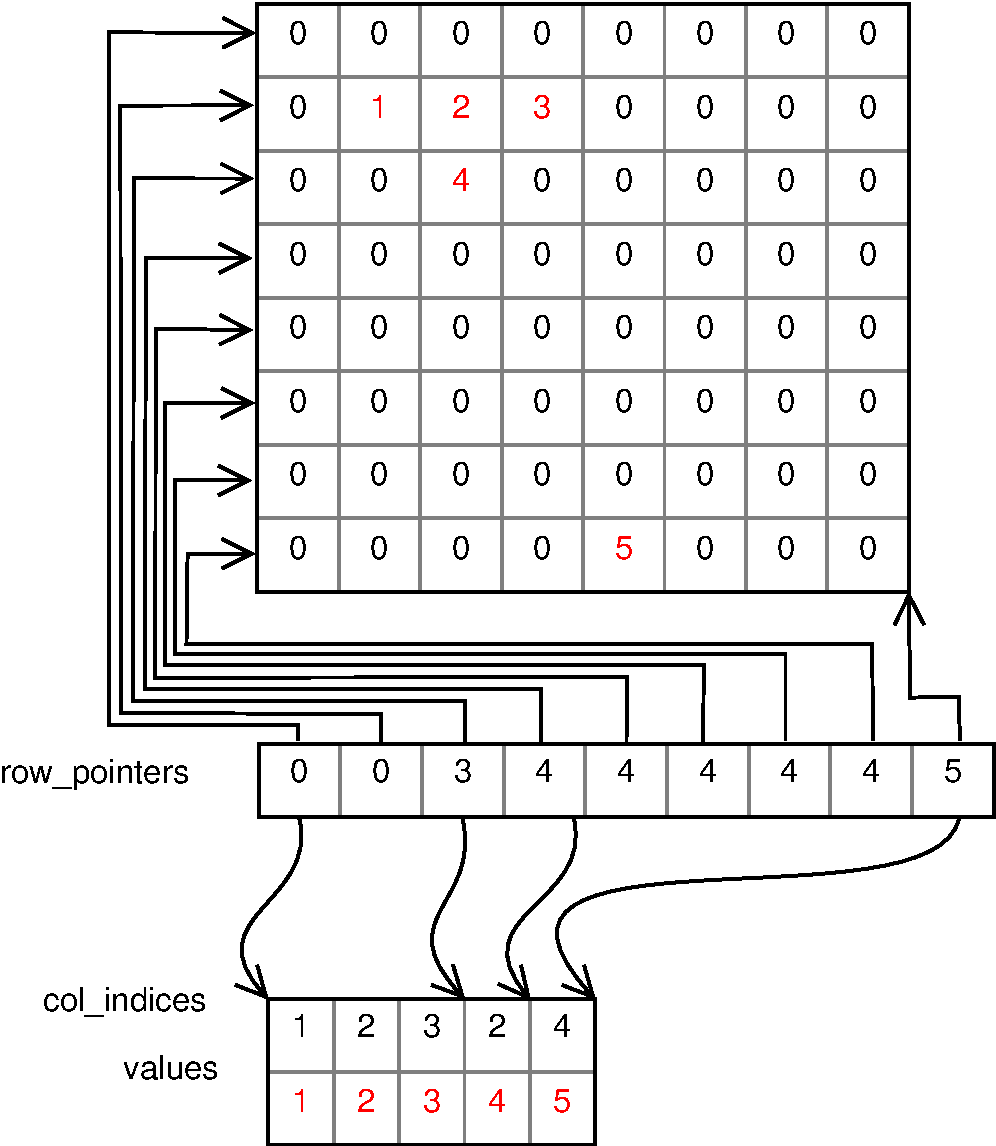
\includegraphics[width=\textwidth]{./images/csr/csr}
	\caption{Matice uložená ve formátu CSR}
	\label{fig:CSR}
\end{figure}

Jak je vidět z ilustrace \ref{fig:CSR}, řádek s více prvky je uložen efektivně. Kvůli mnoha prázdným řádkům se ale pole $row\_pointers$ nezdá rozumně využité.

Při násobení matice CSR s vektorem potřebujeme o jeden for cyklus více než v případě násobení matice COO s vektorem. Důvodem je ztráta informace o řádku prvku.

\begin{algorithm}[htb]
	\caption{Násobení matice CSR s vektorem}\label{csr-mvm}
	\begin{algorithmic}[1]
		\Procedure{CSR-MVM}{CSR,V,C}
		\For{\texttt{i $\gets$ 0 \TO CSR.h}}
			\For{\texttt{ci $\gets$ CSR.rp[i]\TO CSR.rp[i + 1]}}
				\State \texttt{C.v[r] += CSR.v[ci] * V.v[A.ci[ci]];}
			\EndFor
		\EndFor
		\EndProcedure
	\end{algorithmic}
\end{algorithm}

Násobení dvou CSR matic je stejné jako v případě násobení dvou COO matic \ref{fig:CSR}. Jediný rozdíl je, že předpočítané začátky a konce řádků jsou součástí formátu.

\label{alg:csr-mmm}
\begin{algorithm}[htb]
	\caption{Násobení dvou CSR matic}\label{csr-mmm}
	\begin{algorithmic}[1]
		\Procedure{CSR-MMM}{A,B,C}
		\For{\texttt{i $\gets$ 0\TO A.height}}\Comment{násobení}
			\For{\texttt{ac $\gets$ A.rp[i]\TO A.rp[i + 1]}}
				\For{\texttt{bc $\gets$ B.rp[A.ci[ac]]\TO B.rp[A.ci[ac] + 1]}}
					\State \texttt{C.v[r][B.ci[bc]] += A.v[ac] * B.v[bc];}
				\EndFor
			\EndFor
		\EndFor
		\EndProcedure
	\end{algorithmic}
\end{algorithm}

Pro uložení matice ve formátu CSR potřebujeme pole o velikost $n + 1$ pro uložení informací o řádcích a $2 \cdot nnz$ pro prvky a jejich sloupce. Paměťová složitost formátu CSR je \bigO($ n+1 + 2 \cdot nnz $). 

Existuje varianta tohoto formátu, nazvaná CSC - compressed sparse columns, která místo ukládání řádku ukládá sloupce.

\section{BSR - Block Sparse Row}

Jako formát CSR využívá uložení prvků v řádku, formát BSR \cite{bsrscipy}\cite{bsrintel} ještě navíc detekuje a ukládá prvky v blocích.

Protože při násobení matic násobíme každý prvek dvakrát, bylo by dobré tyto dvě operace provést co nejdříve po sobě, abychom při druhém znovu-načtení prvku mohli sáhnout pro prvek do cache. Pokud jsou prvky procházené po menších blocích, dostaneme se k prvku podruhé dříve, než jej z cache přemaže jiný prvek.

Matici $A$ ve formátu BSR ukládáme velice podobně jako u formátu CSR pomocí tří polí. Je potřeba i jedna proměnná, která uchovává velikost bloku. Tuto proměnnou nazveme $block\_size$. Pole $col\_indices$ označuje sloupec, ve kterém se blok nachází. Sloupcem rozumíme blok prvků o šířce \\ $A.width / A.block\_size$.

\begin{figure}[htb]\centering
	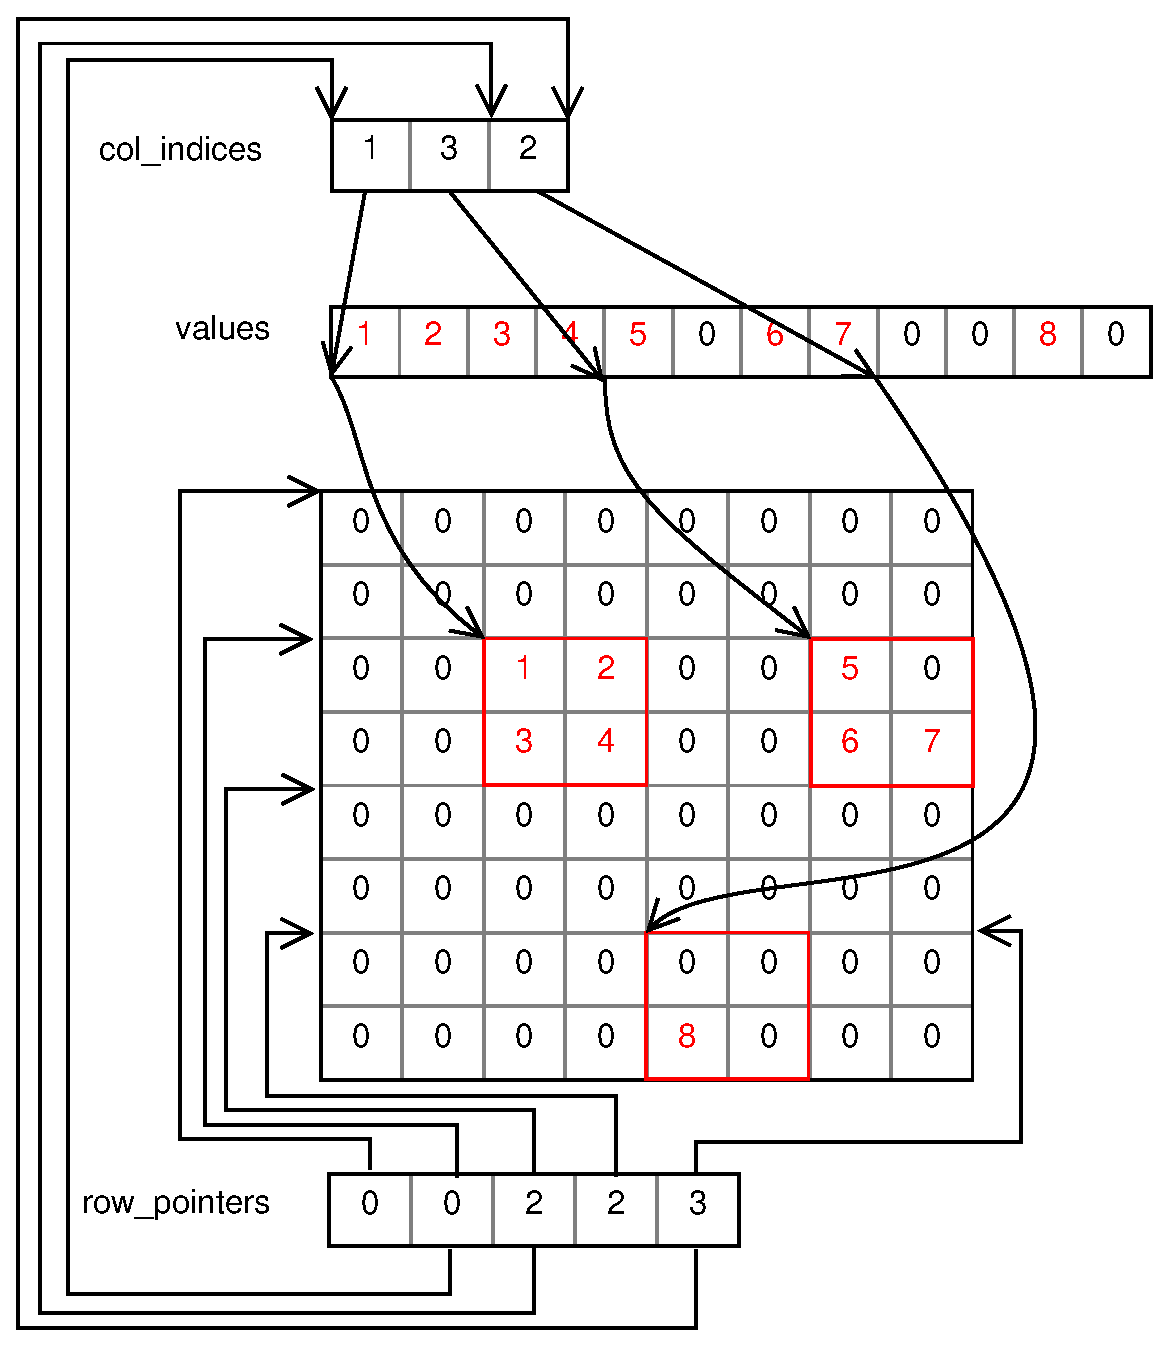
\includegraphics[width=\textwidth]{./images/bsr/bsr}
	\caption{Matice uložená ve formátu BSR}
	\label{fig:BSR}
\end{figure}

Uložení matice ve formátu BSR ilustruje obrázek \ref{fig:BSR}. Pole $row\_pointers$ obsahuje informace o tom, na kterém řádku je kolik bloků. Na řádku $i$ je $row\_pointers[i+1] - row\_pointers[i]$ bloků. Ve kterém sloupci se blok prvků nachází, udává pole $col\_indices$. První blok z řádku $i$ je ve sloupci $col\_indices[$ $row\_pointers[i]]$ a poslední blok je ve sloupci $col\_indices[ row\_pointers[i+1] ]$. Pole $values$ obsahuje prvky v blocích, včetně nulových prvků.

Pokud vezmeme algoritmus násobení dvou CSR matic respektive CSR matice s vektorem, jen místo prvků násobíme bloky, vznikne nám algoritmus pro násobení dvou BSR matric, respektive BSR matice s vektorem. Za povšimnutí stojí větší počet for cyklů s menším rozsahem iterace než u CSR. To nám v nejvnitřnějších cyklech dovoluje lépe využívat cache. Jedná se tedy o přístup podobný optimalizační technice loop tiling\cite{Wolf:1991:DLO:113445.113449}.

\label{alg:bsr-mvm}
\begin{algorithm}[H]
	\caption{Násobení matice BSR s vektorem}\label{bsr-mvm}
	\begin{algorithmic}[1]
		\Procedure{BSR-MVM}{A,B,C}
		\State \texttt{bs $\gets$ A.block\_size;}
		\For{\texttt{i $\gets$ 0\TO A.height / bs}}
			\For{\texttt{ac $\gets$ A.rp[i]\TO A.rp[i + 1]}}
				\For{\texttt{l $\gets$ 0 \TO A.bs}}\Comment{násobení bloku}
					\For{\texttt{m $\gets$ 0\TO bs}}
						\State \texttt{C.v[(i * bs) + l] += A.v[ac * (bs * bs) + (l * bs) + m] * B.v[A.ci[ac] * bs + m];}
					\EndFor
				\EndFor
			\EndFor
		\EndFor
		\EndProcedure
	\end{algorithmic}
\end{algorithm}

\label{alg:bsr-mmm}
\begin{algorithm}[H]
	\caption{Násobení dvou BSR matic}\label{bsr-mmm}
	\begin{algorithmic}[1]
		\Procedure{BSR-MMM}{A,B,C}
		\State \texttt{bs $\gets$ A.block\_size;}
		\For{\texttt{i $\gets$ 0\TO A.height / bs}}
			\For{\texttt{ac $\gets$ A.rp[i]\TO A.rp[i+1]}}
				\For{\texttt{bc $\gets$ B.rp[A.ci[ac]]\TO B.rp[A.ci[ac]+1]}}
					\For{\texttt{l $\gets$ 0\TO A.bs}}\Comment{násobení bloku}
						\For{\texttt{m $\gets$ 0\TO bs}}
							\For{\texttt{n $\gets$ 0\TO bs}}
								\State \texttt{C.v[(i * bs) + l][(B.ci[bc] * bs) + m] += A.v[ac * (bs * bs) + (l * bs) + n] * B.v[bc * (bs * bs) + (n * bs) + m];}
							\EndFor
						\EndFor
					\EndFor
				\EndFor
			\EndFor
		\EndFor
		\EndProcedure
	\end{algorithmic}
\end{algorithm}

Paměťová složitost je závislá na počtu bloků $b$, velikosti bloků $block\_size$ a počtu řádek matice $n$. Pole $row\_pointers$ má velikost $n+1$, pole $col\_indices$ má velikost $b$ a pole hodnot $values$ má velikost $b \cdot sm\_size^2$. Celková velikost matice uložené ve formátu BSR je \bigO$(n + b + b \cdot sm\_size^2)$. 

\section{Quadtree}

Předchozí popsané formáty uložení řídkých matic jsou velmi přímočaré. Neumožňují rekurzivní přístup, který je potřebný například pro Strassenův algoritmus. Tento problém řeší formát Quadtree \cite{JA_SNA_08_QUAD}\cite{qdtsf}. Jedná se o matici uloženou v 4-árním stromě.

Tento formát dělí matici na čtvrtiny do té doby, než se dosáhne velikosti podmatice $sm\_size$, nebo ve čtvrtině nejsou žádné prvky. Pokud je celá čtvrtina prázdná, je uzel označen jako prázdný, $E$. Pokud obsahuje nějaké prvky, je list označen jako hustý, $D$. Vnitřní uzly jsou označeny jako smíšené, $M$.

Obrázek \ref{fig:quad1} ukazuje, že kořen stromu Quadtree představuje celou matici. Jeho synové představují čtvrtinu matice, jak je v obrázku \ref{fig:quad2}. Dělení matice se zastaví, pokud je blok k dělení prázdný, jako například v \ref{fig:quad3}, nebo byla dosažena velikost $sm\_size$.

\begin{figure}[htb]\centering
	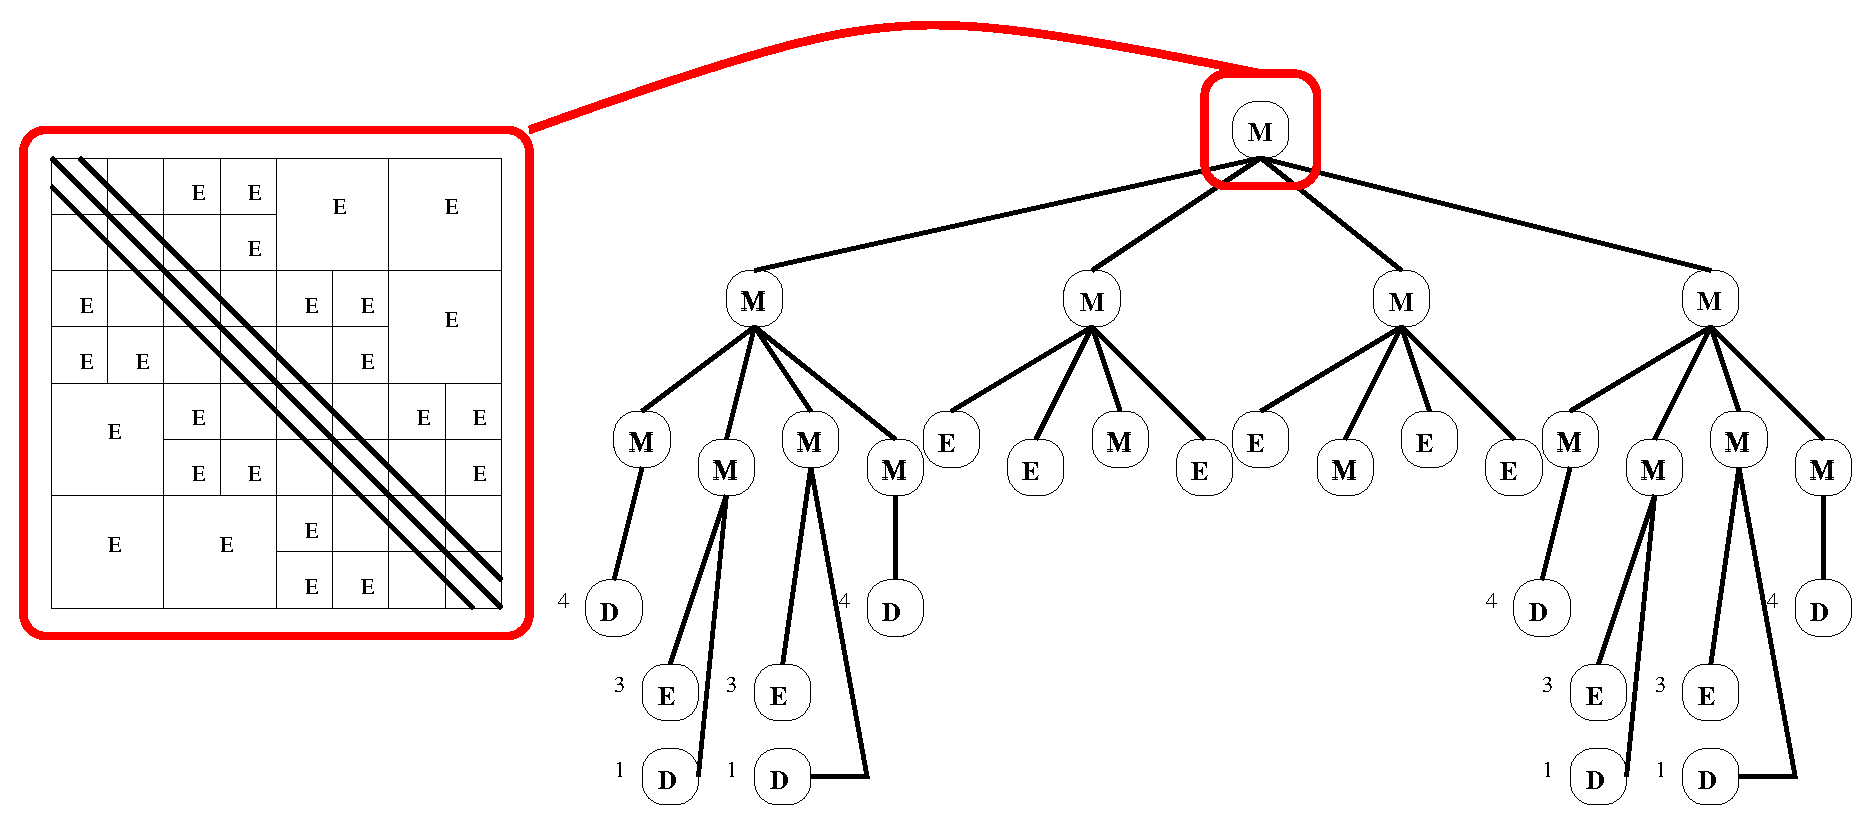
\includegraphics[width=\textwidth]{./images/quadtree_sourceforge/quad2a.eps}
	\caption{Rozdělení matice Quadtree \cite{quadsime}}
	\label{fig:quad1}
\end{figure}

\begin{figure}[htb]\centering
	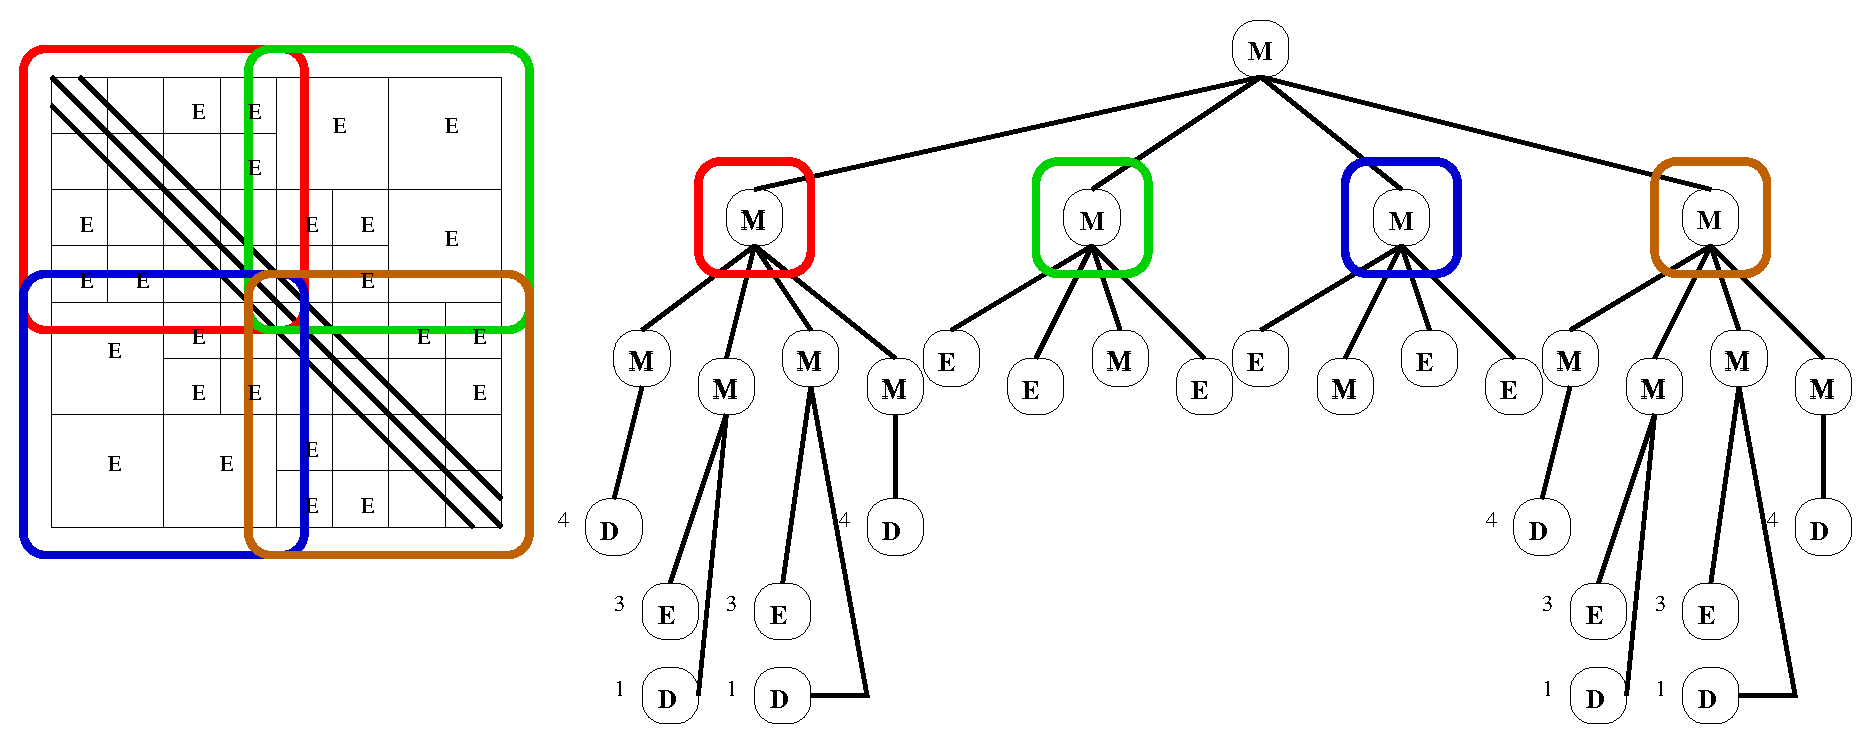
\includegraphics[width=\textwidth]{./images/quadtree_sourceforge/quad2b.eps}
	\caption{Rozdělení matice Quadtree \cite{quadsime}}
	\label{fig:quad2}
\end{figure}

\begin{figure}[htb]\centering
	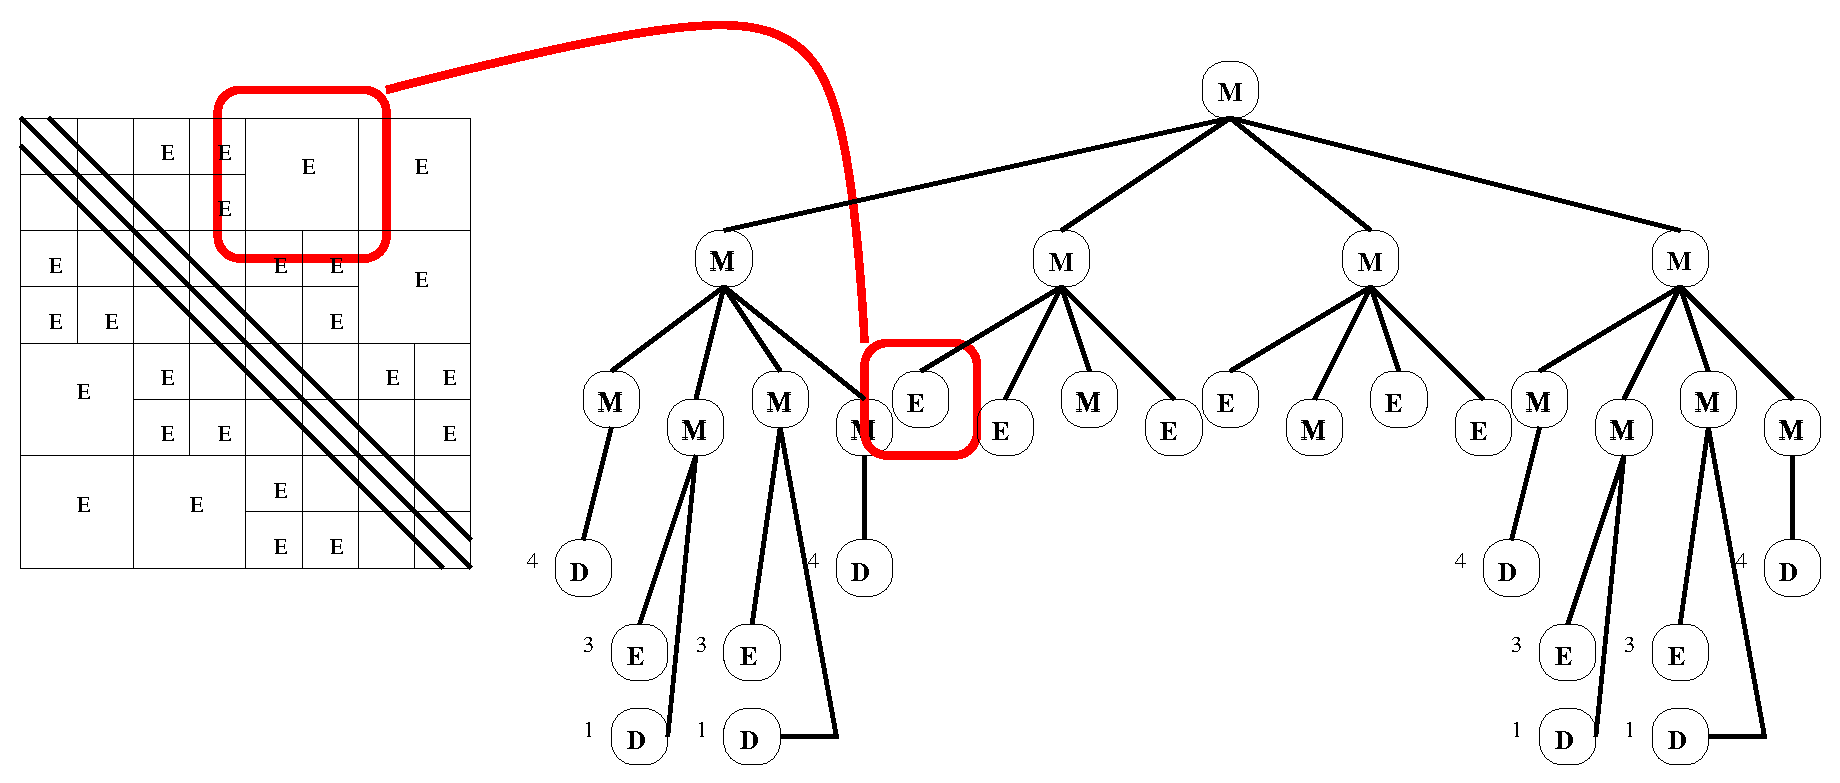
\includegraphics[width=\textwidth]{./images/quadtree_sourceforge/quad2c.eps}
	\caption{Rozdělení matice Quadtree \cite{quadsime}}
	\label{fig:quad3}
\end{figure}


Výška stromu Quadtree je při reprezentaci matice o velikosti $n$ a při velikosti podmatice $sm\_size$:

\label{quadtreeheight}
\begin{align}
\Bigg\lceil\log_{4}\frac{n^2}{sm\_size^2}\Bigg\rceil
\end{align}

\label{quadexampl}
Například pro matici o velikosti $n=16384$ s velikostí bloku $sm\_size=128$ je výška stromu $7$.

Algoritmy pro práci s formátem Quadtree budou ukázány v kapitole o obecnějším formátu \ref{katchapter}.

% \section{?}
%TODO: tady jsem chtel spocictat kdy  se vyplati mit ridkou matici, ale lepsi bude tabulka. Pokud například uložíme matici o %rozměrech 100x100 v dvojté přestnosti, bude zabírat \texttt{M x N x sizeof(double) = 100 x 100 x 8 = 80000B = 80kB}. Pokud zvolíme %řídký formát matice, kde ke každému elementu uložíme i jeho x a y souřadnici, tak do 80kB uložíme \texttt{80000 / %(sizeof(int)+sizeof(int)+sizeof(double)) = 80000/16= 5000} elementů. Pokud matice obsahuje více jak 50  \% nulových elementů, %vyplatí se nám ji uložit do řídkého formátu.

\section{Modifikace formátu quadtree}
\label{katchapter}

V této práci navrhujeme místo 4-árního stromu obecný $k$-ární strom. Výška stromu se tím sníží. Pro předchozí příklad \ref{quadexampl} by tedy pro 16-ární strom byla výška pouze $4$. Tento formát nazveme \texttt{k-ary tree matrix} se zkratkou KAT. Pro přehlednost nebudeme uvádět $k$, ale $KAT.n = sqrt(k)$. Formát Quadtree můžeme prohlásit za matici KAT s $KAT.n = 2$. Pro snadnější rekurzivní přístup budeme jako $KAT.n$ uvažovat pouze mocniny dvou.

Výška stromu pro KAT matici označíme jako \texttt{KAT.height} a vypočítáme ji jako výšku Quadtree, jen s parametrem $k$:

\label{katheight}
\begin{align}
KAT.height = \Bigg\lceil\log_{k}\frac{n^2}{sm\_size^2}\Bigg\rceil
\end{align}

Pokud to bude z kontextu jasné, budeme výšku KAT stromu značit pouze $height$.


\subsection{Typy listů}

KAT matice obsahuje proměnnou $KAT.dense\_treshold$, která udává maximální počet prvků, aby se s listem pracovalo jako s některým z řídkých formátů, tedy COO, CSR, BSR. Při překročení této hranice je list uložen ve formátu husté matice, tedy bude obsahovat i nulové prvky.

%[TODO: ilustrace kat matrix]

\subsection{Násobení}

Pro násobení budeme používat algoritmus rekurzivního násobení popsaného v \ref{RecMul}. Popsaný algoritmus dělí matice na čtvrtiny, jde tedy aplikovat na formát Quadtree. Při násobení matice uložené v $k$-árním stromě budeme násobit matici podmatic o velikosti $k$:

\label{alg:kat-mvm}
\begin{algorithm}[htb]
	\caption{Násobení matice KAT s vektorem}\label{kat-mvm}
	\begin{algorithmic}[1]
		\Procedure{KAT-MVM}{KAT, KAT\_node, VB, VC}
		\For{\texttt{i $\gets$ 0\TO KAT.n}}
			\For{\texttt{j $\gets$ 0\TO KAT.n}}
				\If{\texttt{KAT\_node.childs[i][j] $\neq$ NIL}}
					\If{\texttt{KAT\_node.childs[i][j].type = "submatrix"}}
						\State \texttt{multiplyNode(KAT\_node.childs[i][j], VB, VC);}
						\State \texttt{coninue;}
					\EndIf
					\If{\texttt{KAT\_node.childs[i][j].type = "inner"}}
						\State \texttt{KAT-MVM(KAT,KAT\_node.childs[i][j], VB, VC);}
						\State \texttt{coninue;}
					\EndIf
				\EndIf
			\EndFor
		\EndFor
		\EndProcedure
	\end{algorithmic}
\end{algorithm}

\label{alg:kat-mmm}
\begin{algorithm}[htb]
	\caption{Násobení dvou KAT matic}\label{kat-mmm}
	\begin{algorithmic}[1]
		\Procedure{KAT-MMM}{KATa, KATa\_node, KATb, KATb\_node, C}
		\For{\texttt{i $\gets$ 0\TO KAT.n}}
			\For{\texttt{j $\gets$ 0\TO KAT.n}}
				\For{\texttt{k $\gets$ 0\TO KAT.n}}
					\If{\texttt{KATa\_node.childs[i][k] $\neq$ NIL and KATb\_node.childs[k][j] $\neq$ NIL}}
						\If{\texttt{KAT\_node.childs[i][j].type = "submatrix"}}
							\State \texttt{multiplyNode(KAT\_node.childs[i][j], KAT\_node.childs[i][j], VC);}
							\State \texttt{coninue;}
						\EndIf
						\If{\texttt{KAT\_node.childs[i][k].type = "inner"}}
							\State \texttt{KAT-MMM(KATa,KATa\_node.childs[i][k], KATb,KATb\_node.childs[k][j], C);}
							\State \texttt{coninue;}
						\EndIf
					\EndIf
				\EndFor
			\EndFor
		\EndFor
		\EndProcedure
	\end{algorithmic}
\end{algorithm}

Přesnější asymptotická složitost násobení matic v KAT formátu je vyšší než u předchozích formátů, protože je potřeba připočítat průchod stromem. Pokud převedeme hustou matici do formátu KAT se složitostí násobení dvou listů \bigO($sm\_size^3$), bude asymptotická složitost násobení dvou KAT matic \bigO$((\frac{n^2}{sm\_size} \cdot (height+sm\_size^3))$.

\subsection{Paměťová složitost}

Paměťová složitost celé KAT matice záleží na typu a hustotě uložení dat. Uvedeme zde pouze paměťovou složitost stromu bez listů. Velikost uzlu je pole $k$ ukazatelů na syny. Počet vnitřních uzlů spočítáme pomocí geometrické posloupnosti. Paměťová složitost stromu KAT matice tedy je \bigO$(\frac{k^{height-1}-1}{k - 1} \cdot k)$ po zkrácení \bigO$(k^{height-2}-k-\frac{1}{k})$.